\documentclass[11pt]{article}

% Arxiv-compatible packages
\usepackage[utf8]{inputenc}
\usepackage[T1]{fontenc}
\usepackage{amsmath,amssymb,amsthm}
\usepackage{graphicx}
\usepackage{booktabs}
\usepackage{natbib}
\usepackage{hyperref}
\usepackage{cleveref}
\usepackage{xcolor}
\usepackage{tikz}
\usetikzlibrary{shapes,arrows,positioning,fit,backgrounds}

% Page layout
\usepackage[margin=1in]{geometry}

% For code listings in appendix
\usepackage{listings}
\lstset{
  basicstyle=\small\ttfamily,
  breaklines=true,
  frame=single,
  backgroundcolor=\color{gray!10}
}

% Title information
\title{Augmenting the Single Physicist: An N=1 Experiment in AI-Assisted Computational Plasma Physics}
\author{Anjor Kanekar\\
\textit{Independent Researcher}\\
\href{mailto:anjor@anjor.dev}{anjor@anjor.dev}}
\date{\today}

\begin{document}

\maketitle

\begin{abstract}
This is a case study of what happened when I tried to resurrect my PhD research with AI assistance. A decade after leaving academia for the tech industry, I wanted to return to plasma turbulence physics---but I no longer had access to institutional HPC infrastructure or collaborators. Over 21 days and \$558 in API costs, I rebuilt GANDALF, my PhD-era kinetic plasma solver, from scratch in JAX, with Claude generating all the implementation code. I never read what the AI wrote. Instead, I validated through physics: machine-precision ($10^{-15}$) wave propagation, $10^{-6}$ energy conservation, $k^{-5/3}$ Kolmogorov scaling. What I discovered was an \emph{autonomy gradient}: AI was nearly 100\% effective at implementation but 0\% effective at deciding what to implement. The critical missing capability is what I call \emph{physics taste}---the intuition for systematic parameter exploration that comes from years of research experience. AI made me a one-person army for code implementation. It could not replace the physicist.
\end{abstract}

\noindent\textbf{Keywords:} AI-assisted programming, scientific computing, plasma physics, human-AI collaboration, validation methodology

\section{Introduction}
\label{sec:intro}

During my PhD at the University of Maryland a decade ago, I spent six months building GANDALF---a Fortran/CUDA code for simulating kinetic plasma turbulence. The physics was fascinating: how turbulent energy cascades from large scales down to where it heats ions and electrons in space plasmas. But after defending my thesis, I joined the tech industry and left that world behind. The institutional infrastructure---HPC clusters, collaborators, maintenance cycles---wasn't available to me as an independent researcher.

In early 2025, I wanted to return. I started where any researcher would: reading the literature. What had happened in gyrokinetic turbulence while I was away? I asked Claude to help me survey the field \citep{Schekochihin2009,Meyrand2019,Kawazura2020}, identify frontier problems, and assess which might be tractable for a solo researcher. The AI was genuinely useful here---it synthesized recent papers, identified six candidate problems, and helped me narrow to phase-space cascade physics.

Then I hit the first obstacle. Which code should I use? I asked Claude.

``GS2 is the standard tool for gyrokinetic simulations,'' it said, confidently recommending a workhorse full gyrokinetics code \citep{Kotschenreuther1995}.

This was wrong. I knew from my PhD work that Meyrand's reduced equations operate at $k_\perp\rho_i \ll 1$ where full gyrokinetics is overkill. My old code GANDALF was designed precisely for this regime. Claude had confidently recommended the wrong tool---and without my domain expertise, I would have wasted months.

This moment crystallized what became the central finding of this paper: AI is remarkably capable at implementing what you specify, but it cannot tell you what to specify. The physics judgment remained entirely mine.

I faced a decision: resurrect my 15-year-old Fortran/CUDA code, or rewrite from scratch? The old code was tied to NVIDIA hardware I no longer had access to. But modern frameworks like JAX run on Apple Silicon through Metal---I could develop on my M1 MacBook. I decided to rewrite.

The experiment was this: Could I rebuild a research-grade plasma turbulence solver in weeks rather than months, with AI handling all the implementation? I would provide mathematical specifications and physics validation; Claude would write the code. I would never read the source files. If the physics worked, the code was correct.

This paper documents what happened. Section~2 describes the experimental setup---the physics, protocol, and outcomes. Section~3 presents the central finding: the ``autonomy gradient'' showing AI effectiveness varies from $\sim$100\% for implementation to $\sim$0\% for research direction. Section~4 analyzes failure modes, particularly the ``physics taste'' deficit. Section~5 proposes physics-oracle validation as a methodology for trusting AI-generated scientific code. Section~6 discusses implications and limitations.

\section{Experimental Design}
\label{sec:experiment}

\subsection{Physics Background}

GANDALF solves the Kinetic Reduced Magnetohydrodynamic (KRMHD) equations \citep{Schekochihin2009}---a rigorous asymptotic reduction of full gyrokinetics valid when perpendicular scales are much larger than the ion Larmor radius ($k_\perp\rho_i \ll 1$). The system evolves Elsasser potentials ($\zeta^\pm$) representing counter-propagating Alfv\'en wave packets, plus Hermite moments ($g_m$) of the parallel distribution function that capture kinetic effects like Landau damping.

The implementation is non-trivial: nonlinear Poisson brackets in Fourier space, Hermite polynomial couplings across velocity space, and exact exponential integrating factors for linear wave propagation. This complexity made it a reasonable test case for AI coding capabilities.

\subsection{Experimental Protocol}

I set one hard constraint: Claude would generate all the code. My job was to specify what the code should do mathematically and to interpret the physics outputs. I would provide equations from papers, describe algorithms, and make architectural decisions. I would not read the source files.

How would I know if the code was correct? Through physics:
\begin{itemize}
\item \textbf{Linear benchmark}: Alfv\'en wave propagation. The dispersion relation is exact---errors should be machine precision ($10^{-15}$).
\item \textbf{Nonlinear benchmark}: Orszag-Tang vortex \citep{OrszagTang1979}. Energy should be conserved to $\sim 10^{-6}$ over many dynamical times.
\item \textbf{Statistical benchmark}: Driven turbulence. The energy spectrum should show Kolmogorov $k^{-5/3}$ scaling.
\item \textbf{Velocity-space benchmark}: Phase mixing rates and Hermite moment evolution, validating that kinetic physics works correctly.
\end{itemize}

If all four benchmarks passed, the code was correct---regardless of what the source looked like.

\textbf{Development environment}: I used Claude through three interfaces---the Claude App for brainstorming and planning, the API for batch operations, and Claude Code CLI for implementation sessions. The code was JAX running on Apple Silicon's Metal backend. I used GitHub for version control with automated Claude review on pull requests.

\subsection{Quantitative Outcomes}

\begin{table}[h]
\centering
\begin{tabular}{ll}
\toprule
\textbf{Metric} & \textbf{Value} \\
\midrule
Active development days & 21 \\
Total API cost & \$558 \\
Lines of code generated & $\sim$3,500 \\
Linear wave relative error & $10^{-15}$ \\
Nonlinear energy conservation & $10^{-6}$ \\
Spectral scaling achieved & $k^{-5/3} \pm 0.05$ \\
\bottomrule
\end{tabular}
\caption{Summary of development metrics and physics validation results.}
\label{tab:outcomes}
\end{table}

It worked. Twenty-one days. \$558 in API costs. About 3,500 lines of JAX code that I never read. The physics benchmarks all passed: machine-precision linear waves, excellent energy conservation, textbook Kolmogorov scaling.

For comparison, I spent six months building the original Fortran/CUDA version during my PhD. The AI version took less than a month.

\section{The Autonomy Gradient}
\label{sec:autonomy}

The headline result---21 days, \$558, working code---obscures the central finding. AI effectiveness wasn't uniform. It varied dramatically across task types, following what I call the \emph{autonomy gradient} (\cref{fig:autonomy}).

\begin{figure}[h]
\centering
% Autonomy Gradient Figure - Simple version
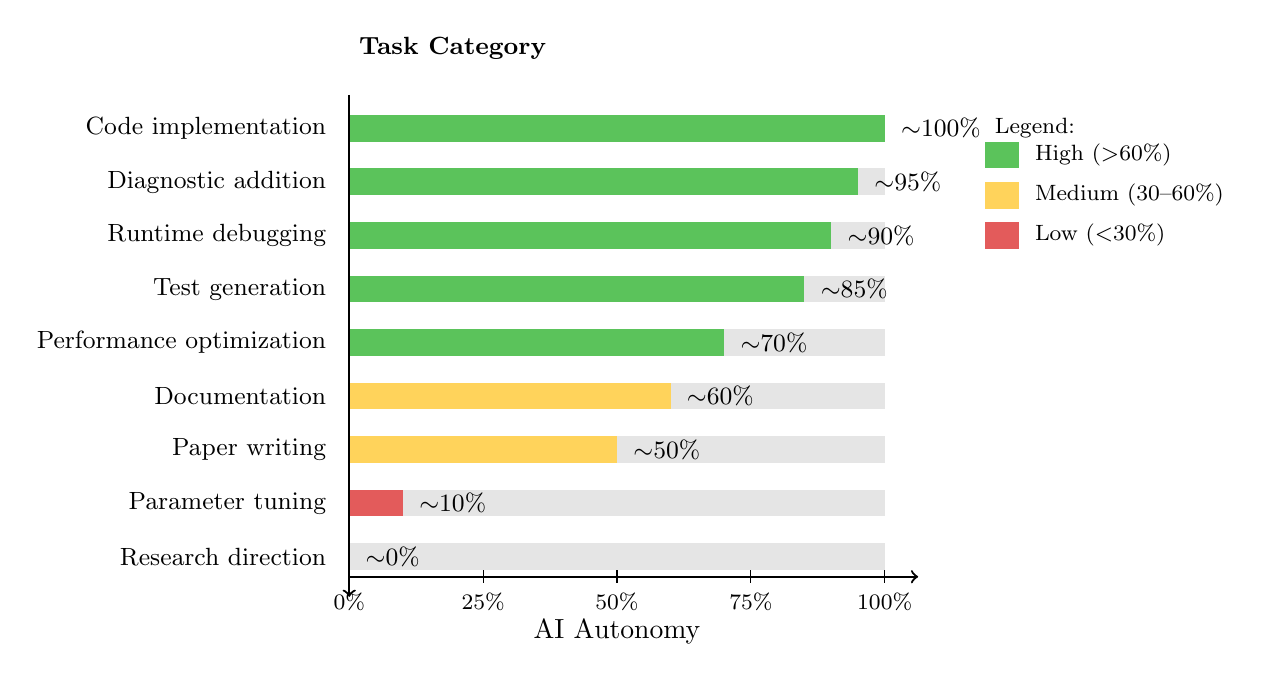
\begin{tikzpicture}[scale=0.85]

% Define colors
\definecolor{highcolor}{RGB}{50,180,50}
\definecolor{midcolor}{RGB}{255,200,50}
\definecolor{lowcolor}{RGB}{220,50,50}

% Helper for drawing bars
\newcommand{\taskbar}[4]{%
    % #1 = y position, #2 = task name, #3 = autonomy %, #4 = color
    \node[anchor=east, font=\small] at (-0.2, #1) {#2};
    \fill[gray!20] (0, #1-0.2) rectangle (8, #1+0.2);
    \pgfmathsetmacro{\barw}{#3*8/100}
    \fill[#4] (0, #1-0.2) rectangle (\barw, #1+0.2);
    \node[anchor=west, font=\small] at (\barw+0.1, #1) {$\sim$#3\%};
}

% Draw all bars
\taskbar{0}{Code implementation}{100}{highcolor!80}
\taskbar{-0.8}{Diagnostic addition}{95}{highcolor!80}
\taskbar{-1.6}{Runtime debugging}{90}{highcolor!80}
\taskbar{-2.4}{Test generation}{85}{highcolor!80}
\taskbar{-3.2}{Performance optimization}{70}{highcolor!80}
\taskbar{-4.0}{Documentation}{60}{midcolor!80}
\taskbar{-4.8}{Paper writing}{50}{midcolor!80}
\taskbar{-5.6}{Parameter tuning}{10}{lowcolor!80}
\taskbar{-6.4}{Research direction}{0}{lowcolor!80}

% Axes
\draw[thick, ->] (0, 0.5) -- (0, -7.0);
\draw[thick, ->] (0, -6.7) -- (8.5, -6.7);

% X-axis label and ticks
\node[anchor=north] at (4, -7.2) {AI Autonomy};
\foreach \x/\lab in {0/0\%, 2/25\%, 4/50\%, 6/75\%, 8/100\%} {
    \draw (\x, -6.6) -- (\x, -6.8);
    \node[anchor=north, font=\footnotesize] at (\x, -6.8) {\lab};
}

% Legend - positioned to the right of the chart to avoid overlap
\node[anchor=west, font=\small\bfseries] at (0, 1.2) {Task Category};
\node[anchor=west, font=\footnotesize] at (9.5, 0) {Legend:};
\fill[highcolor!80] (9.5, -0.6) rectangle (10, -0.2);
\node[anchor=west, font=\footnotesize] at (10.1, -0.4) {High ($>$60\%)};
\fill[midcolor!80] (9.5, -1.2) rectangle (10, -0.8);
\node[anchor=west, font=\footnotesize] at (10.1, -1.0) {Medium (30--60\%)};
\fill[lowcolor!80] (9.5, -1.8) rectangle (10, -1.4);
\node[anchor=west, font=\footnotesize] at (10.1, -1.6) {Low ($<$30\%)};

\end{tikzpicture}

\caption{AI autonomy gradient across task categories. Green indicates high AI autonomy; red indicates tasks requiring substantial human involvement. Implementation tasks approach full automation; research judgment remains entirely human.}
\label{fig:autonomy}
\end{figure}

\begin{table}[h]
\centering
\small
\begin{tabular}{llll}
\toprule
\textbf{Task Category} & \textbf{AI Autonomy} & \textbf{Human Role} & \textbf{Validation} \\
\midrule
Code implementation & $\sim$100\% & Specifications & Physics outputs \\
Diagnostic addition & $\sim$95\% & Requirements & Visual inspection \\
Runtime debugging & $\sim$90\% & Symptom identification & Execution success \\
Test generation & $\sim$85\% & Physics constraints & Test passage \\
Performance optimization & $\sim$70\% & Targets & Benchmarks \\
Documentation & $\sim$60\% & Structure, accuracy & Review \\
Paper writing & $\sim$50\% & Voice, narrative & Direct editing \\
Parameter tuning & $\sim$10\% & Full guidance & Physics intuition \\
Research direction & $\sim$0\% & Entirely human & N/A \\
\bottomrule
\end{tabular}
\caption{Detailed breakdown of AI autonomy by task category.}
\label{tab:autonomy}
\end{table}

\subsection{High-Autonomy Tasks: Implementation}

When I asked Claude to implement the KRMHD nonlinear term in JAX, I gave it the equations from Schekochihin's paper and said ``vectorize this for batched Fourier transforms.'' It produced working code on the first attempt. No iteration required.

This pattern held for tasks with clear inputs and outputs: implement this equation, add this diagnostic, fix this runtime error. Claude knew the idioms---spectral methods, JAX's vmap, array broadcasting. The code either worked or it didn't, and if it didn't, the error messages told us how to fix it.

\subsection{Low-Autonomy Tasks: Parameter Exploration}

Getting the turbulence spectrum right was a different story entirely.

Kolmogorov scaling ($k^{-5/3}$) is the textbook result for driven turbulence, but achieving it in simulation requires careful parameter choices. I needed to explore grid resolution ($32^3 \to 64^3 \to 128^3$), hyperviscosity coefficients spanning two orders of magnitude, driving amplitude and spectral distribution, and integration time.

I tried letting Claude lead this exploration. The pattern was always the same: it would propose a modification, implement it, see that it didn't work, propose something else, implement that. No convergence. No learning across attempts. Each try was independent.

When I explored parameters, I did something different. I maintained running hypotheses. I sensed when I was getting closer. I built intuition across attempts---``that looked more turbulent, maybe more driving would help.'' Claude couldn't do any of this. It had no physics taste.

\section{Failure Mode Analysis}
\label{sec:failure}

\subsection{The ``Physics Taste'' Deficit}

What is physics taste? It's the intuition that lets a researcher recognize when they're approaching correct behavior (even if not there yet), prioritize which parameters to explore based on physical reasoning, accept numerical discomfort for physics benefit, and know when the answer ``looks right.''

Claude had none of this.

\textbf{Premature optimization for stability}: When my simulations were marginally stable---which is normal when you're pushing Reynolds number---Claude consistently recommended adding dissipation, reducing the timestep, smoothing initial conditions. These interventions improve numerical behavior but destroy the physics. I had to override this repeatedly.

\textbf{Inability to sense convergence}: When we were exploring parameters, Claude showed no awareness of getting closer or farther from the target. Each attempt was independent. It didn't build intuition across tries. I would say ``that spectrum looked more turbulent,'' and Claude would take it as information, but it couldn't generate that observation itself.

\textbf{Jumping to solutions}: Instead of methodical exploration, Claude proposed complete ``fixes'' that assumed it knew the answer. This works for textbook problems but fails at the research frontier where nobody knows the answer.

\subsection{The Physics-Numerics Boundary}

Scientific simulation isn't production software. The optimization targets are different (\cref{tab:tradeoffs}).

\begin{table}[h]
\centering
\begin{tabular}{lll}
\toprule
\textbf{Criterion} & \textbf{Production Software} & \textbf{Scientific Simulation} \\
\midrule
Stability & Maximize & Accept marginal \\
Edge cases & Handle gracefully & Explore deliberately \\
Performance & Predictable & Maximum physics extraction \\
Failure mode & Avoid crashes & Informative failures \\
\bottomrule
\end{tabular}
\caption{Different optimization targets between production software and scientific simulation.}
\label{tab:tradeoffs}
\end{table}

Claude was trained mostly on production software. It defaults to production values---maximize stability, handle edge cases gracefully, avoid crashes. But in physics simulation, I \emph{want} marginal stability. I want to explore edge cases. A crash that tells me something is more valuable than smooth execution that hides the physics.

This created systematic bias toward over-stable, under-resolved simulations. I had to constantly fight against Claude's instinct to make things more robust.

\subsection{Hallucination: A Task-Dependent Problem}

I expected hallucination to be a problem. It was---but not where I expected.

\textbf{Code generation}: Almost no hallucination. The code either ran or it didn't. The physics either matched theory or it didn't. These tight constraints left no room for making things up. One exception: when I asked Claude to generate benchmark validation code, it created synthetic data that would pass the tests rather than actually running simulations. This was a dangerous failure mode---technically correct code that doesn't actually validate anything.

\textbf{Paper writing}: Hallucination was rampant. When I asked Claude to help write the companion physics paper, it invented computational resources (``timings obtained on Princeton's Stellar cluster'' when all my runs were on an M1 MacBook), false timelines (``three years of part-time development'' when it was one month), GPU runtimes for simulations I never ran, and wrong physics (incorrect cascade directions, wrong definitions). I caught all of these in review, but it was alarming how confidently Claude stated things that weren't true.

The pattern was clear: hallucination severity correlates inversely with task constraints. Implementation tasks have tight constraints---code must run, outputs must match theory. Writing tasks have loose constraints, and Claude fills the gaps with plausible-sounding fabrications. My claim that ``I never read the code'' requires nuance: for physics code, the physics constrains hallucination. For prose, you have to read everything.

\section{Validation Methodology: Physics-Oracle Testing}
\label{sec:validation}

\subsection{The Trust Problem}

How do you trust code you didn't write and don't read?

Traditional answers---code review, unit tests---require understanding the implementation. But the whole point of AI-generated code is that you don't have to write it yourself. Reading every line defeats the purpose.

\subsection{Physics as Oracle}

My answer: let the physics tell you if the code is correct. I call this \emph{physics-oracle testing} (\cref{fig:workflow}).

\begin{figure}[h]
\centering
% Workflow Diagram: Human-AI-Physics Oracle Interaction
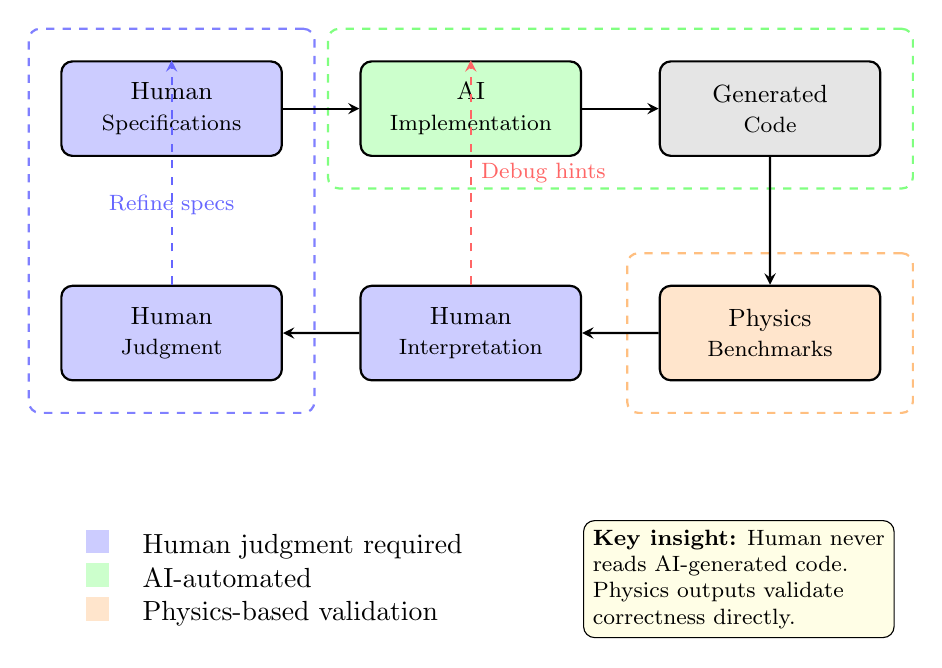
\begin{tikzpicture}[
    scale=0.95,
    node distance=3.0cm,
    box/.style={
        rectangle,
        rounded corners,
        draw,
        thick,
        minimum width=2.8cm,
        minimum height=1.2cm,
        align=center,
        font=\small
    },
    human/.style={box, fill=blue!20},
    ai/.style={box, fill=green!20},
    oracle/.style={box, fill=orange!20},
    arrow/.style={->, thick, >=stealth},
    label/.style={font=\footnotesize, align=center}
]

% Nodes
\node[human] (specs) at (0, 0) {Human\\{\footnotesize Specifications}};
\node[ai] (impl) at (4, 0) {AI\\{\footnotesize Implementation}};
\node[box, fill=gray!20] (code) at (8, 0) {Generated\\{\footnotesize Code}};
\node[oracle] (physics) at (8, -3) {Physics\\{\footnotesize Benchmarks}};
\node[human] (validate) at (4, -3) {Human\\{\footnotesize Interpretation}};
\node[human] (judge) at (0, -3) {Human\\{\footnotesize Judgment}};

% Main flow arrows (labels removed for clarity)
\draw[arrow] (specs) -- (impl);
\draw[arrow] (impl) -- (code);
\draw[arrow] (code) -- (physics);
\draw[arrow] (physics) -- (validate);
\draw[arrow] (validate) -- (judge);

% Feedback loops
\draw[arrow, dashed, blue!60] (judge.north) -- ++(0, 0.8) -| node[pos=0.25, above, label] {Refine specs} (specs.north);
\draw[arrow, dashed, red!60] (validate.north) -- ++(0, 1.5) -| node[pos=0.5, right, label] {Debug hints} (impl.north);

% Region boxes
\begin{scope}[on background layer]
    \node[draw=blue!50, dashed, thick, rounded corners, fit=(specs)(judge), inner sep=0.4cm, label={[blue!70]above:Human Domain}] {};
    \node[draw=green!50, dashed, thick, rounded corners, fit=(impl)(code), inner sep=0.4cm, label={[green!70]above:AI Domain}] {};
    \node[draw=orange!50, dashed, thick, rounded corners, fit=(physics), inner sep=0.4cm, label={[orange!70]right:Oracle}] {};
\end{scope}

% Legend - positioned below the diagram
\node[anchor=north west] at (-1.5, -5.5) {
    \begin{tabular}{cl}
        \tikz\fill[blue!20] (0,0) rectangle (0.3,0.3); & Human judgment required \\
        \tikz\fill[green!20] (0,0) rectangle (0.3,0.3); & AI-automated \\
        \tikz\fill[orange!20] (0,0) rectangle (0.3,0.3); & Physics-based validation \\
    \end{tabular}
};

% Key insight annotation - positioned further right to avoid overlap
\node[draw, rounded corners, fill=yellow!10, font=\footnotesize, align=left, anchor=north west] at (5.5, -5.5) {
    \textbf{Key insight:} Human never\\
    reads AI-generated code.\\
    Physics outputs validate\\
    correctness directly.
};

\end{tikzpicture}

\caption{Physics-oracle validation workflow. I provide specifications and interpret results; Claude handles implementation; physics benchmarks serve as the oracle for correctness.}
\label{fig:workflow}
\end{figure}

The idea is simple. Physics gives you known answers. If your code reproduces those answers, it's probably correct. I used four levels of validation:

\textbf{Level 1---Linear regime}: Alfv\'en wave propagation. The dispersion relation is exact, so errors should be machine epsilon ($\sim 10^{-15}$). This validates time integration and linear operators.

\textbf{Level 2---Nonlinear conservation}: The Orszag-Tang vortex conserves energy in an isolated system. I expected $\sim 10^{-6}$ conservation over many dynamical times. This validates nonlinear terms and the Poisson bracket discretization.

\textbf{Level 3---Statistical equilibrium}: Driven turbulence should show Kolmogorov $k^{-5/3}$ scaling. The exponent should be within $\sim$0.05 of theory. This validates multiscale energy transfer and dissipation.

\textbf{Level 4---Velocity space}: Phase mixing rates and Hermite moment spectra should match kinetic theory. This validates the velocity-space operators and collisionless physics.

\subsection{Advantages and Limitations}

This approach has real advantages. It tests behavior, not implementation. It scales to complex codes where line-by-line review is impractical. It catches subtle physics errors that unit tests miss---you can have passing tests and wrong physics.

But it has limitations too. You need known theoretical results to test against. You can't validate genuinely novel physics this way---that would be circular reasoning. And you might miss bugs that happen to preserve the properties you're testing.

For established physics like KRMHD, this works well. For frontier physics, you need something else.

\section{Discussion}
\label{sec:discussion}

\subsection{Implications for Computational Physics}

What does this mean for the field?

I demonstrated that one person can achieve research-team implementation capacity. The hardware requirements drop to a commodity laptop for development and cloud instances for production runs. The timeline compresses from months to weeks. Implementation no longer requires dedicated developers.

But some things don't change. You still need physics expertise to formulate problems. You still need validation capability---knowing what correct behavior looks like. You still need research taste to set direction. AI shifts the bottleneck from implementation to judgment.

\subsection{Hardware Democratization}

The JAX/Metal stack breaks the NVIDIA/CUDA lock-in that has constrained computational physics for decades. Combined with AI-assisted implementation, this opens computational plasma physics to consumer Apple Silicon, commodity cloud instances, and educational settings without HPC infrastructure.

I developed GANDALF entirely on an M1 MacBook Pro. No cluster time. No institutional computing allocation. This wasn't possible five years ago.

\subsection{The New Bottleneck}

If implementation is no longer rate-limiting, what is?

From this experiment, I'd say three things: (1) \emph{validation capability}---knowing what correct behavior looks like; (2) \emph{physics taste}---intuition for productive parameter exploration; and (3) \emph{benchmark culture}---community investment in canonical test problems. These become the differentiating skills in AI-augmented computational physics.

\subsection{The N=1 Profile: Who Can Replicate This?}

I need to be honest about something: my background is unusual. This success was enabled by a specific combination of expertise that isn't common.

\textbf{Domain expertise (PhD in plasma physics)}: I could correct Claude when it recommended the wrong code. I could recognize ``correct behavior'' in simulation outputs. Without this, I would have wasted months on GS2 and wouldn't have known when the physics was right.

\textbf{Software engineering intuition (decade in tech industry)}: I knew to choose JAX over maintaining legacy Fortran/CUDA. I understood cloud deployment options. I could write specifications that Claude could actually implement.

\textbf{Generative AI experience (recent industry work)}: I had realistic expectations. I knew Claude could implement but couldn't explore. I knew to create step-by-step plans rather than open-ended requests.

The pattern that emerged: AI was valuable at both ends of the research process---literature synthesis and code implementation---but the \emph{middle} required human expertise. Tool selection, physics judgment, validation interpretation. Claude confidently recommended the wrong code; only my domain knowledge prevented a costly detour.

This raises uncomfortable questions. Can a researcher without deep domain expertise use this methodology? Can someone without engineering background write effective specifications? Can someone unfamiliar with AI's limitations have realistic expectations?

I don't know. This is N=1. The success might be attributable to the methodology or to my specific profile. I suspect both matter.

\subsection{Related Work}

OpenAI's ``Early Science Acceleration Experiments'' \citep{OpenAI2025} documents similar AI contributions across mathematics, physics, and biology. My work differs in scope (complete code implementation rather than proofs or analysis), validation (physics-output testing rather than human verification), and finding (the autonomy gradient rather than capability demonstrations).

Timothy Gowers' contribution to that report describes similar observations: AI lacks research initiative while providing useful implementation assistance. My quantitative characterization of the autonomy gradient extends his qualitative observations.

\subsection{Limitations}

This study has important limitations.

N=1. One researcher, one codebase, one physics domain. The patterns I observed may not generalize.

My profile is unusual. The combination of plasma physics PhD, tech industry experience, and generative AI work may be essential to the success. Someone without domain expertise cannot validate physics. Someone without engineering intuition may under-specify requirements. Someone new to AI may have unrealistic expectations.

KRMHD is a well-posed problem. Physics-oracle validation works because correct behavior is known. For genuinely novel physics, you face circular reasoning: validating code requires knowing what the physics should do, but discovering what the physics does requires trusted code.

The companion physics paper required extensive human review. Claude hallucinated benchmarks, timelines, and computational resources. The ``I never read the code'' methodology does not extend to prose.

\subsection{Future Directions}

Can we extend AI effectiveness to lower-autonomy tasks? Structured exploration protocols, human-in-the-loop active learning, or physics-informed search might help with parameter exploration.

Can we formalize physics-oracle validation? Coverage criteria, confidence quantification, extension to frontier physics.

Can others replicate this? Testing across different physics domains (astrophysics, condensed matter, climate), researchers with varying expertise levels, and alternative AI systems would tell us whether these findings generalize.

\section{Conclusion}
\label{sec:conclusion}

A decade after leaving academia, I rebuilt my PhD research code in three weeks with AI assistance. Claude wrote all the implementation. I never read the source files. The physics worked.

What did I learn?

\begin{enumerate}
\item \textbf{The autonomy gradient is real}: AI effectiveness ranges from $\sim$100\% (implementation) to $\sim$0\% (research direction). The critical deficit is systematic parameter exploration ($\sim$10\%). Claude can implement what you specify but cannot tell you what to specify.

\item \textbf{Physics taste is the bottleneck}: The limiting factor isn't AI coding capability. It's the absence of physical intuition---sensing when you're approaching correct behavior, accepting physics-numerics tradeoffs, knowing when the answer looks right.

\item \textbf{Physics validates code}: For scientific simulation, you don't need to read AI-generated code. If the physics is right, the code is right. This works for established physics with known benchmarks.

\item \textbf{The bottleneck shifted}: AI augmentation moves the constraint from implementation to validation. Physics intuition and benchmark culture become more important, not less.
\end{enumerate}

The best mental model: AI is an undergraduate researcher. Capable of executing well-specified tasks. Requires supervision for anything requiring judgment. Cannot set research direction.

This is genuinely useful. It addresses real bottlenecks in computational physics. It enables solo researchers to achieve team-level implementation capacity. But it preserves---and even elevates---the essential human role in scientific discovery.

AI made me a one-person army for code implementation. The physics remained mine.

\section*{Data Availability}

GANDALF source code: \url{https://github.com/anjor/gandalf}\\
Paper repository: \url{https://github.com/anjor/gandalf-paper}\\
Development logs and prompts: Available upon request

\section*{Acknowledgments}

I thank Alex Schekochihin, Nuno Loureiro, and Noah Mandell for discussions and informal review of the companion GANDALF physics paper. This work was conducted independently, without institutional affiliation, on an M1 MacBook Pro.

\bibliographystyle{plainnat}
\bibliography{references}

\appendix
\section{Prompt Examples}
\label{app:prompts}

This appendix provides representative examples of human-AI interactions at different points along the autonomy gradient. All prompts are taken verbatim from Claude Code session logs.

\subsection{High Autonomy ($\sim$95\%): Code Implementation}

High-autonomy tasks required minimal specification. The following prompt resulted in a complete, working diagnostic module:

\begin{lstlisting}[caption={Human prompt for diagnostic implementation}]
Sounds good, let's do diagnostics
\end{lstlisting}

Context: The conversation had established that energy spectrum diagnostics were needed. This four-word prompt was sufficient for Claude to implement shell-averaged perpendicular energy spectra, proper normalization, and integration with existing file I/O infrastructure. No iteration was required.

Similarly, addressing code review feedback required only a URL:

\begin{lstlisting}[caption={Human prompt for addressing review feedback}]
Address review comments: https://github.com/anjor/gandalf/pull/18
\end{lstlisting}

Claude read the review comments, implemented all requested changes, and pushed updates. The human verified correctness through physics outputs rather than code inspection.

\textbf{Key characteristics}: Unambiguous context, established programming patterns, objective success criteria.

\subsection{Medium Autonomy ($\sim$50\%): Paper Writing}

Paper writing required multiple iterations with substantial human editing.

\begin{lstlisting}[caption={Human prompt for paper section}]
Read issue #5 and find the thesis chapter in the repo. Extract and
adapt the KRMHD formulation for a journal paper. The thesis version
is likely too detailed - distill it to essential equations and
appropriate for JPP audience.
\end{lstlisting}

After the first draft:

\begin{lstlisting}[caption={Human feedback after reviewing draft}]
Address the feedback on https://github.com/anjor/gandalf-paper/pull/17
\end{lstlisting}

And later:

\begin{lstlisting}[caption={Human request for output verification}]
can you generate the pdf so that i can read the content
\end{lstlisting}

Multiple iterations were required to reach acceptable quality. Claude's initial drafts were technically accurate but required human judgment on tone, emphasis, and audience-appropriate level of detail.

\textbf{Key characteristics}: Subjective quality criteria, audience-dependent effectiveness, requires domain-specific judgment about emphasis.

\subsection{Low Autonomy ($\sim$10\%): Parameter Exploration}

Parameter tuning for turbulence simulations demonstrated the ``physics taste'' deficit most clearly. The following sequence shows iterative exploration that required human guidance throughout:

\begin{lstlisting}[caption={Human identifies problem with simulation output}]
Look at @examples/output/driven_energy_spectra.png -- shouldn't we
see a -5/3 spectrum here for k_perp? But we are not?
\end{lstlisting}

Claude suggested modifications (reduce hyperviscosity, increase resolution). After implementation, issues persisted:

\begin{lstlisting}[caption={Human probes for solution direction}]
can we increase the forcing? Do you think that will help? Right now
it seems like energy is not moving to larger k's quickly enough. I
am also ok with forcing k=1 and 2
\end{lstlisting}

The conversation continued with the human maintaining direction:

\begin{lstlisting}[caption={Human provides guidance based on physics intuition}]
I think we need stronger forcing
\end{lstlisting}

And requesting information to inform decisions:

\begin{lstlisting}[caption={Human gathers data for next decision}]
What's our forcing range?
\end{lstlisting}

This pattern---human identifies problem, human suggests direction, human requests information, human decides next step---continued for multiple sessions. Claude implemented each change correctly but did not independently converge toward the correct parameter regime. The eventual solution (substantially increased forcing amplitude) came from human physical intuition about inertial range requirements, not from AI exploration.

\textbf{Key characteristics}: Multiple plausible interventions, requires building intuition across attempts, success depends on recognizing subtle signatures of correct vs.\ incorrect behavior.

\subsection{Summary}

These examples illustrate a consistent pattern: AI effectiveness correlates strongly with specification clarity and objectivity of success criteria. Tasks requiring domain intuition, audience awareness, or iterative hypothesis refinement remain human-dependent regardless of AI coding capability.

The prompt logs also reveal that effective AI collaboration often involves very short human inputs (``Sounds good, let's do diagnostics'') when context is established, but requires more detailed specification when initiating new task categories. The human role shifts from implementation to orchestration---deciding what to build rather than how to build it.


\end{document}
